\renewcommand{\thepage}{}
\chapter{Problem Statement}
\thispagestyle{empty}
\pagestyle{fancy}
\lhead{\small \bf  Chapter 1: Problem Statement}
\rhead{}
\chead{}
\renewcommand\thepage{\arabic{page}}
 \setcounter{minitocdepth}{1}
\minitoc
 
\newpage
\section{Introduction}
\lettrine[lines=2,lhang=0.44,lraise=0,loversize=0.08,findent=-0.11em,slope=0.6em]%
{I}{} nformation is always the critical success factor of key of strategic decisions. The fast growing market of mobile devices as smart phones and tablets changes drastically the picture and offer new way of working. These mobile devices overwhelm the population and might become the preferred computing tools. Information becomes mobile.
The increased use of mobile computing has imposed a new challenge: the ability to represent information of any kind on smaller devices. It is in this context that the idea of radial representation of data structures organized as trees and graphs is born. The company Stradefi-SA, which we present in the following paragraph, had an urgent need to achieve a 3-tier architecture based application capable of managing data organized in the form of graphs and trees.
This application, which is intended for an intensive use by intermediate of mobile devices, must support the radial representation of these
data structures.
  
\section{Company's presentation}
\paragraph*{}
\textbf{Stradefi-SA} is a privately owned company in Geneva specialized in highly secured. It servers the content management, Business process and customer relation. Works in private Cloud Mobile Computing architecture. Stradefi`s consultants delivered innovative solution to companies as:Novartis, PNB PARIBAS, Romande Energie
\section{Project issues}
\paragraph*{}
In the real life a lot of relationships exist between different entities. An entity may be a physical person or any kind of object. These relations may be unilateral, bilateral, or multiple. Every single object could have relations with hundreds of other entities.
\paragraph*{}
To automate the management of entities and their relationships, and in order to process them by computers, one must represent them as abstractions. One of the most active areas in the IT domain is "Graph and Tree" representation [1]. In the Graph Theory, a Graph is a representation of a set of objects where some pairs of objects are connected by links.
\paragraph*{}
Formally, a Graph [1] is a pair G = (V, E) of sets, where V is the set of vertices, such that $E = [V]�$ formed by pairs of vertices. formed by pairs of vertices. E is a multiset, in other words, its elements can occur more than once so that every element has a multiplicity [2].
\paragraph*{}
A directed graph (or digraph) [W3] in mathematics, and more specifically in graph theory,is a graph, or set of nodes connected by edges, where the edges have a direction associated with them. A set V, whose elements are called vertices or nodes, and a set E of ordered pairs of vertices, called arcs, directed edges, or arrows (and sometimes simply edges with the corresponding set named E). It differs from an ordinary or undirected graph, in that the latter is defined in terms of unordered pairs of vertices, which are usually called edges. This(figure-1) illustrate a Directed Graph:
\vspace*{2mm}
\begin{figure}[h]
\begin{center}
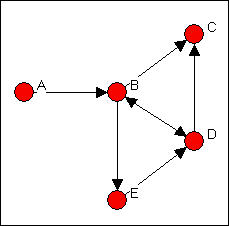
\includegraphics[scale=0.5, frame]{Figure_1.jpg}
\end{center}
\caption{Directed Graph}
\end{figure}
\paragraph*{}
In the theory there is no restrictions on the number of relations that a certain node may have.
Depending on the piece of the displayed graph, the node may appear disconnected as illustrated in (figure-2):
\begin{figure}[h]
\begin{center}
\includegraphics[scale=0.5]{tel11.png}
\end{center}
\caption{Usual graphical representation of a graph/tree}
\label{Figure of Simple Graph Representation}
\end{figure}
\paragraph*{}
The work that has been achieved is intended to manage the presentation of Graph in a way that avoids the problems described above.
\section{Project summary}
\paragraph*{}
Customers of \textbf{Stradefi SA} usually are Pharmaceutical Laboratories, Private Banks, Medical Cabinets, etc. This kind of organizations manage lots of entities as well as relationships between them. For example a customer of a private bank may have different accounts of different types.
\paragraph*{}
He also may have some bank advisers. He may have a shared account with his wife, etc. The customer, his wife, the adviser and the different account are seen as entities that are bound by relationships:
\begin{itemize}
\item the customer owns the accounts,
\item the customer has a wife,
\item the customer is advised by a bank employee,
\item etc.
\end{itemize}
\paragraph*{}
It is, therefore natural to abstract and represent the entities and their relations in the form of Graphs as we have already mentioned that in the introduction. The work present on this report is to implement an application that covers the need to manage entities that have relations with each other and implemented in the form of Graphs. We have identified through a technical interview with the customers, and from there business our objectives.
\subsection{Proposed solution}
\paragraph*{}
Referring to the issues that have been exposed in $�1.3$ the classical visualization of graphs and trees is not suitable to mobile devices. We, therefore, have investigated other kinds of these data structures visualization that combine simplicity and efficiency. We found out that the radial representation is the solution to these issues. 
\paragraph*{}
The radial layout encodes directed graphs on narrow rings of a circle [3]. The hierarchical evolution of the graph is mapped to rings that grow outward from the center of the circle. Graph vertices are placed equidistantly at the borderlines of each ring. Graph edges are displayed as curved lines starting from a source on the inner borderline of the ring and pointing to a target on the outer borderline. To better perceive link directions and structures of large data-sets, visual clutter is reduced by exploiting an edge splatting approach that generates density felds of the displayed edges. The radial layout emphasizes newer graphs, displayed in the larger, outer parts of the circle. As a benefit, edge lengths are reduced in comparison to the non-radial visualization. Moreover, the radial layout guarantees the symmetry of the visualization under shifting of vertices.
\begin{figure}[h]
\begin{center}
\includegraphics[scale=0.5]{tel22.png}
\end{center}
\caption{Radial Form}
\label{Figure of Radial Representation}
\end{figure}
\section{Conclusion}
\paragraph*{}
In this chapter we have discussed the issues related to data visualization on mobile devices, especially data that is formalized in the form of graphs and trees. We have also presented the motivation of Stradefi-SA to implement a solution that covers all of these problems. Potential customers exist and there is a real need that has been expressed trough technical interviews conducted by the company.
\paragraph*{}
The challenge was to chose between two alternatives: implement an application from the scratch or use an already existing library that is capable of the radial visualization. This will be discussed in the following chapter: "state of the art".
